\documentclass[dvipsnames]{standalone}
\usepackage[utf8]{inputenc}
\usepackage{tikz}
\usepackage{pgfplots}
\usepackage{pgfkeys}
\usetikzlibrary{shadows.blur, arrows}
\usetikzlibrary{calc}
\title{tikz-pt}
\author{dexter2206 }
\date{January 2023}


\pgfplotsset{compat=1.18} 
\begin{document}

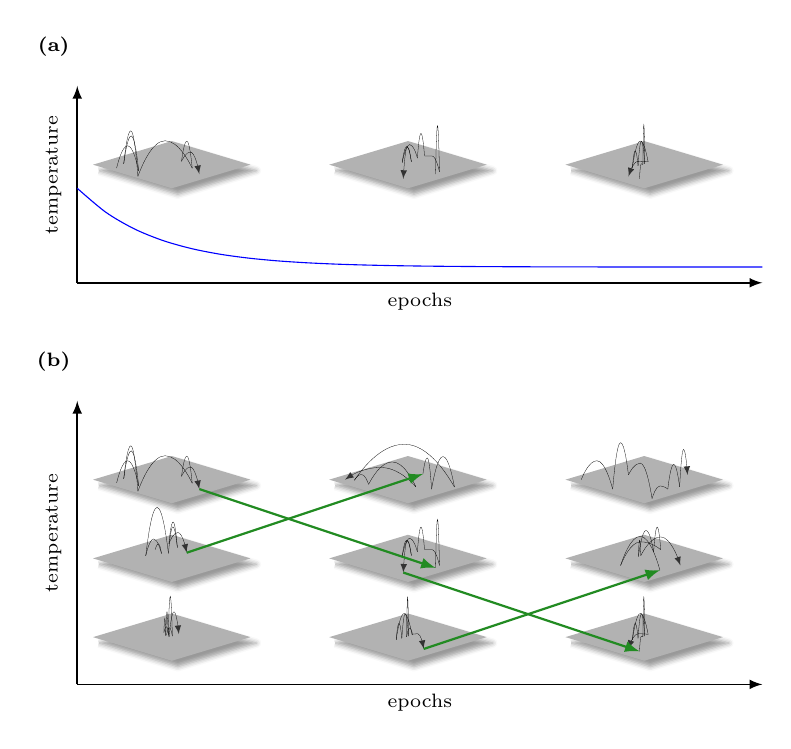
\begin{tikzpicture}[
    x={(1cm,0.0cm)}, 
    y={(0,0.3cm)}, 
    z={(0cm,1cm)}, 
    statespace/.style={
        fill=black!30!white, opacity=1, blur shadow
    },
    exchange/.style={color=ForestGreen,thick,-latex}
]

\newcommand{\point}[1]{(#1[0], #1[1], 0)}


\tikzset {
    heights/.store in = \heights,
    states/.store in = \states,
    statespace/.pic={
        \tikzset{#1}
        \fill[statespace] 
            (-1, 0, 0) -- (0,-1,0) -- (1,0,0) -- (0,1,0) -- (-1,0,0);
        \pgfmathparse{dim(\heights)-1}
        \let\lasti\pgfmathresult
        \foreach \i in {0,...,\pgfmathresult}
        {
          \ifnum\i=\lasti
            {\draw[ultra thin,-latex] 
                \point{{\states}[\i]} 
                parabola[parabola height={{\heights}[\i]}]
                \point{{\states}[\i+1]};
            }            
          \else{\draw[ultra thin] \point{{\states}[\i]} parabola[parabola height={{\heights}[\i]}] \point{{\states}[\i+1]};}
          \fi
         }     
          %\else
          %\fi
    }
}

% Replicas in first epoch
\path (-1.5, 0, 1) pic{
        statespace={
            heights={
                0.3cm, 
                0.4cm, 
                0.5cm, 
                0.4cm, 
                0.3cm, 
                0.2cm
            },
            states={
                {-0.7,-0.14},
                {-0.42,-0.26},
                {-0.61,0.03},
                {-0.43,-0.49},
                {0.26,-0.15},
                {0.124,0.14},
                {0.35,-0.4}
            }
        } 
    }
      (-1.5, 0, 0) pic{
        statespace={
            heights={
                0.1cm, 
                0.2cm, 
                0.6cm, 
                0.3cm, 
                0.3cm,
                0.2cm
            },
            states={
                {-0.21,0.37},
                {-0.13,0.2},
                {-0.33,0.11},
                {-0.042,0.21},
                {0.071,0.46},
                {-0.036,0.62},
                {0.19,0.24}
            }
        }
    }
      (-1.5, 0, -1) pic{
        statespace={
            heights={0.1cm, 0.5cm, 0.3cm, 0.2cm, 0.1cm, 0.3cm},
            states={
                {-0.067,0.076},
                {0.0076,0.045},
                {-0.045,0.077},
                {-0.076,0.06},
                {-0.1,0.2},                
                {-0.034,0.0132},
                {0.09,0.13},
            }
        }
    };

% Replicas in second epoch
\path (1.5, 0, 1) pic{
        statespace={
            heights={
                0.3cm, 0.4cm, 0.5cm, 0.1cm, 0.3cm, 0.2cm
            },
            states={
                {0.19,0.24},
                {0.3,-0.4},
                {0.59,-0.31},
                {-0.68,-0.024},
                {-0.5,-0.2},
                {0.1,-0.3},
                {-0.8, 0.0}
            }
        }
    }
      (1.5, 0, 0) pic{
        statespace={
            heights={0.6cm, 0.1cm, 0.3cm, 0.2cm, 0.2cm, 0.3cm},
            states={
                {0.35,-0.4},
                {0.4,-0.3},
                {0.21,0.37},
                {0.12,0.28},
                {-0.074,0.086},
                {0.043,0.12},
                {-0.06,-0.6}
            }
        }
    }
      (1.5, 0, -1) pic{
        statespace={
            heights={0.1cm, 0.5cm, 0.3cm, 0.2cm, 0.3cm, 0.1cm},
            states={
                {0.06,0.09},
                {-0.017,0.013},
                {0.0078,0.038},
                {-0.078,-0.048},
                {-0.15,-0.12},
                {0.05,0.12},
                {0.2, -0.5}
            }
        }
    };

% replicas in the third epoch
\path (4.5, 0, 1) pic{
        statespace={
            heights={
                0.3cm, 0.5cm, 0.3cm, 0.1cm, 0.3cm, 0.4cm
            },
            states={
                {-0.8, 0.0},
                {-0.4, -0.4},
                {-0.2, 0.2},
                {0.1, -0.8},
                {0.3,-0.4},
                {0.45,-0.31},
                {0.55, 0.2}
            }
        }
    }
      (4.5, 0, 0) pic{
        statespace={
            heights={0.4cm, 0.2cm, 0.3cm, 0.3cm, 0.2cm, 0.3cm},
            states={
                {0.2, -0.5},
                {-0.3,-0.3},
                {0.21,0.37},
                {0.12,0.28},
                {-0.074,0.086},
                {-0.043,0.12},
                {0.46,-0.3}
            }
        }
    }
      (4.5, 0, -1) pic{
        statespace={
            heights={0.1cm, 0.5cm, 0.3cm, 0.2cm, 0.3cm, 0.1cm},
            states={
                {-0.06,-0.6},
                {-0.017,0.013},
                {0.0078,0.038},
                {-0.078,-0.048},
                {-0.15,-0.12},
                {0.05,0.12},
                {-0.2, -0.5}
            }
        }
    };

% Visualize the exchange
\draw[exchange] (-1.15, -0.4, 1) -- (1.85, -0.4, 0);
\draw[exchange] (-1.31, 0.24, 0) -- (1.69, 0.24, 1);
\draw[exchange] (1.7, -0.5, -1) -- (4.7,-0.5, 0);
\draw[exchange] (1.44,-0.6, 0) -- (4.44,-0.6, -1);

% Draw coordinate system
\draw[-latex,semithick] 
    (-2.7, 0, -1.6) -- (6, 0, -1.6) 
    node[midway, below, font=\scriptsize] {epochs};
\draw[-latex,semithick] 
    (-2.7, 0, -1.6) -- (-2.7, 0, 2) 
    node[
        midway, 
        left, 
        rotate=90, 
        xshift=1cm, 
        font=\scriptsize, 
        yshift=0.3cm
    ] {temperature};

\path (-1.5, 0, 5) pic{
        statespace={
            heights={
                0.3cm, 
                0.4cm, 
                0.5cm, 
                0.4cm, 
                0.3cm, 
                0.2cm
            },
            states={
                {-0.7,-0.14},
                {-0.42,-0.26},
                {-0.61,0.03},
                {-0.43,-0.49},
                {0.26,-0.15},
                {0.124,0.14},
                {0.35,-0.4}
            }
        } 
    }
          (1.5, 0, 5) pic{
        statespace={
            heights={0.6cm, 0.1cm, 0.3cm, 0.2cm, 0.2cm, 0.3cm},
            states={
                {0.35,-0.4},
                {0.4,-0.3},
                {0.21,0.37},
                {0.12,0.28},
                {-0.074,0.086},
                {0.043,0.12},
                {-0.06,-0.6}
            }
        }
    }
    (4.5, 0, 5) pic{
        statespace={
            heights={0.1cm, 0.5cm, 0.3cm, 0.2cm, 0.3cm, 0.1cm},
            states={
                {-0.06,-0.6},
                {-0.017,0.013},
                {0.0078,0.038},
                {-0.078,-0.048},
                {-0.15,-0.12},
                {0.05,0.12},
                {-0.2, -0.5}
            }
        }
    }
    ;

\draw[-latex,semithick] 
    (-2.7, 0, 3.5) -- (6, 0, 3.5) 
    node[midway, below, font=\scriptsize] {epochs};
\draw[-latex,semithick] 
    (-2.7, 0, 3.5) -- (-2.7, 0, 6) 
    node[
        midway, 
        left, 
        rotate=90, 
        xshift=1cm, 
        font=\scriptsize, 
        yshift=0.3cm
    ] {temperature};

\draw[scale=1, domain=-2.7:6, smooth, variable=\x, blue] plot ({\x}, 0, {3.7+exp(-\x-2.7)});

% Finally, some labels

\node[font=\bfseries\scriptsize] at (-3, 0, 6.5) {(a)};
\node[font=\bfseries\scriptsize] at (-3, 0, 2.5) {(b)};
\end{tikzpicture}
\end{document}
